\documentclass[border=6pt]{standalone}
\usepackage{tikz}\usetikzlibrary{positioning,arrows.meta,fit,backgrounds,calc}
\usepackage[T1]{fontenc}\usepackage{lmodern}
\definecolor{slate}{RGB}{48,56,68}\definecolor{accent}{RGB}{198,102,36}\definecolor{mute}{RGB}{120,128,138}
\begin{document}
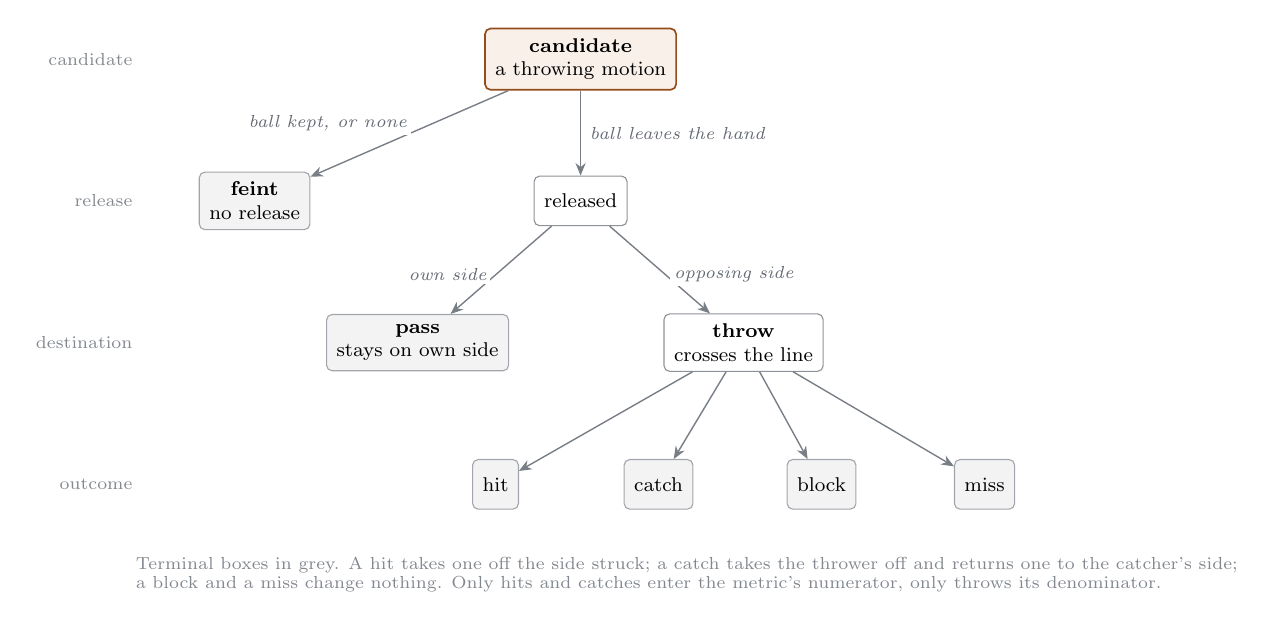
\begin{tikzpicture}[
  scale=0.9, every node/.style={transform shape},
  font=\small,
  lvl/.style={font=\scriptsize, text=slate!60, anchor=east},
  node/.style={draw=slate!55, fill=white, rounded corners=2pt, inner sep=4pt,
               minimum height=7mm, align=center, font=\footnotesize},
  cand/.style={node, draw=accent!75!black, fill=accent!10, line width=0.6pt},
  term/.style={node, draw=slate!45, fill=slate!6},
  q/.style={font=\scriptsize\itshape, text=slate!75, fill=white, inner sep=1.5pt},
  ar/.style={-{Stealth[length=1.6mm,width=1.3mm]}, draw=slate!65, line width=0.5pt},
]
\node[cand] (c) at (0,0) {\textbf{candidate}\\a throwing motion};

\node[term] (fake) at (-4.6,-2.0) {\textbf{feint}\\no release};
\node[node] (rel)  at (0,-2.0)  {released};

\node[term] (pass) at (-2.3,-4.0) {\textbf{pass}\\stays on own side};
\node[node] (thr)  at (2.3,-4.0)  {\textbf{throw}\\crosses the line};

\node[term] (hit)   at (-1.2,-6.0) {hit};
\node[term] (catch) at (1.1,-6.0)  {catch};
\node[term] (block) at (3.4,-6.0)  {block};
\node[term] (miss)  at (5.7,-6.0)  {miss};

\draw[ar] (c) -- (fake) node[q, pos=0.5, above left=-1pt] {ball kept, or none};
\draw[ar] (c) -- (rel)  node[q, pos=0.5, right=2pt] {ball leaves the hand};
\draw[ar] (rel) -- (pass) node[q, pos=0.55, left=2pt] {own side};
\draw[ar] (rel) -- (thr)  node[q, pos=0.55, right=2pt] {opposing side};
\draw[ar] (thr) -- (hit);
\draw[ar] (thr) -- (catch);
\draw[ar] (thr) -- (block);
\draw[ar] (thr) -- (miss);

\node[lvl] at (-6.2,0)    {candidate};
\node[lvl] at (-6.2,-2.0) {release};
\node[lvl] at (-6.2,-4.0) {destination};
\node[lvl] at (-6.2,-6.0) {outcome};

\node[font=\scriptsize, text=slate!60, align=left, anchor=north west] at (-6.4,-6.9)
  {Terminal boxes in grey. A hit takes one off the side struck; a catch takes the thrower off
   and returns one to the catcher's side;\\ a block and a miss change nothing. Only hits and
   catches enter the metric's numerator, only throws its denominator.};
\end{tikzpicture}
\end{document}
